\documentclass[aps,prb,twocolumn,floatfix,nofootinbib,superscriptaddress]{revtex4-2}

\usepackage{amsmath,amssymb,amsthm,mathtools,bm}
\usepackage{booktabs}
\usepackage{graphicx}
\usepackage[colorlinks=true,linkcolor=blue,citecolor=blue,urlcolor=blue]{hyperref}
\usepackage{microtype}

\newcommand{\tr}{\operatorname{tr}}
\newcommand{\ii}{\mathrm{i}}
\newcommand{\code}[1]{\texttt{#1}}
\newcommand{\Geng}{\Gamma}

\graphicspath{
  {../results/N16x20_frozen_flux_charge_v1/figures/}
  {../results/N16x20_frozen_record_continuous_ramp_s10_v1/analysis/figures/}
  {../results/N16x20_frozen_record_fixed_flux_quench_s10_v1/analysis/figures/}
  {../results/N20x24_parent_schrodinger_rk4_s50_tau1e4_v1/analysis/figures/}
  {../../../../notebooks/flattened_hamiltonian_analysis/outputs/exact_wall_charge_pump_refined_v1/run_20260901_002219/figures/}
  {../../../../notebooks/flattened_hamiltonian_analysis/outputs/exact_wall_charge_pump_reversibility_v1/run_20260901_162444/}
}

\hypersetup{
  pdftitle={Wall-Charge Transport under Flux: Exact Benchmark and Monitored-Circuit Ramps},
  pdfauthor={Asadullah Bhuiyan}
}

\begin{document}

\title{Wall-Charge Transport under Flux:\
Exact Benchmark, Static Response, and Monitored-Circuit Ramps}
\author{Asadullah Bhuiyan}
\affiliation{Class-A fermionic adaptive-circuit project}
\date{September 13, 2026}

\begin{abstract}
We collect the present numerical evidence for wall-resolved charge transport
under a threaded boundary flux and specify the next monitored-circuit test.
For the exact flattened Chern-insulator Hamiltonian, an independently filled
instantaneous ground state closes after one flux quantum, whereas overlap
continuation through the wall crossing transfers almost one fermion between
the two interfaces.  At $20\times40$, the continued soft-wall response is
$q_x=0.98397186$ for increasing flux and $-0.99999998$ for decreasing flux;
the hard-wall values are $0.98080970$ and $-1.00000000$.  A completed
$16\times20$ monitored-circuit experiment instead imposed one fixed Born
record in independent static-twist replays.  It displays an order-one,
direction-sensitive conditional response, with maximum $|q_x|=0.62807$ for
the soft wall and $0.43335$ for the hard wall, but closes at $2\pi$ and is not
a dynamical pump.  A completed ten-trajectory online pilot subsequently
branched each cycle-40 burn-in state into independently Born-sampled
clockwise and counterclockwise ramps.  We now preregister a paired conditional
test froze one zero-flux continuation record from each verified burn-in state
and replayed it continuously along both flux orientations for $M=16,32,64$
cycles.  Its direction-odd endpoint decreases with $M$, rather than settling
to a nonzero adiabatic value.  We therefore preregister a fixed-flux quench:
the same burn-in frame and 64-cycle record are replayed with every OW
measurement held at one of four signed twists, including
$2\pi-10^{-7}$.  This directly tests the transient response of a conditioned
measurement channel without tangent-mode tracking.  A separate state-derived
Hamiltonian experiment on 50 saved $20\times24$ endpoints has now completed.
Finite-time RK4 evolution at $T=10^4$ gives raw endpoint means $+0.71569$
(CCW) and $-0.71422$ (CW) for the soft wall, and $+0.53622$ and $-0.53624$
for the hard wall.  Its planned $24\times24$ width repeat was stopped with
zero completed paths and 28 exact rolling checkpoints preserved at interval
104.  We now preregister an adaptive Kato experiment at both widths.  It
removes physical ramp time, defines the spectral branch by previous-projector
overlap, and reports raw CW and CCW transfer separately; no Kato result is
claimed here.  A later wall-diabatized spectral calculation is now complete
for 1600 monitored endpoint states.  Across its 3200 raw directional paths,
98.3\% have the correct orientation and $|q_x|>0.9$, while 97.5\% lie within
$0.95\leq|q_x|\leq1.05$.  This final calculation is a spectral-flow property
of flattened endpoint projectors, not a real-time monitored pump.
\end{abstract}

\maketitle
\setcounter{tocdepth}{2}
\onecolumngrid
\tableofcontents
\twocolumngrid

\section{Purpose and claim structure}

Threading a flux through a cylinder supplies a direct test of chiral boundary
transport in a Chern insulator~\cite{Laughlin1981,Halperin1982}.  In an
equilibrium Hamiltonian, the relevant adiabatic object is a continuously
transported occupied subspace.  In a monitored adaptive circuit, the state is
instead changed by Born-conditioned measurements and fermionic feedback, so a
static family, an online ramp, and modular-time packet propagation answer
different questions.  This working note keeps those distinctions explicit.

The evidence is organized in complementary layers.  First, the exact flattened
Hamiltonian provides a controlled equilibrium benchmark.  Second, the
completed frozen-record calculation measures the circuit's conditional static
response.  Third, the completed $S=10$ experiment makes the twist time
dependent inside one physical monitored trajectory while independently
sampling its directional branches.  Fourth, the continuous frozen-record
ramp holds the complete measurement record fixed while changing only the flux
path.  Fifth, the fixed-flux quench defined below removes the ramp and tests
the transient conditioned channel at four signed twists.  Sixth, a completed
finite-difference unitary experiment evolves saved circuit endpoints under
their state-derived parent Hamiltonians.  Seventh, the newly preregistered
Kato calculation transports the overlap-selected spectral projector directly
in flux.  Eighth, the completed wall-diabatized width sweep isolates the
physical wall doublet from ordinary spectator states and preserves its entering
wall label through the finite-size crossing.  These constructions answer
different physical questions and their outputs are not silently pooled.

\section{Common geometry and charge observable}

The physical cylinder has two orbitals per unit cell, is open in $x$, and is
periodic in $y$.  A topological slab with parent-Hamiltonian parameter
$\alpha_1=1$ is embedded in a trivial exterior with $\alpha_2=30$.  We use the
overcomplete Wannier (OW) basis with trial family $X$ and
$n_{\mathrm{shell}}=1$.  Distinct OW number stabilizers need not commute, and
the OW modes form a localized overcomplete frame rather than an orthonormal
Wannier basis~\cite{BhuiyanPanJian2026}.

Let $G$ be the physical single-particle correlation matrix,
\begin{equation}
  G_{ij}=\operatorname{Tr}
  (\hat\rho\,\hat c_i^\dagger\hat c_j),
  \qquad
  G=\frac{\mathbf{1}+\Geng}{2},
\end{equation}
where $\Geng$ is the centered covariance used by the numerical engine.  The
cylinder is divided into the disjoint half-system regions $R_L$ and $R_R$.
For a path beginning at flux $\phi_0$, define
\begin{align}
  \Delta N_a(\phi)&=\tr[R_aG(\phi)]-\tr[R_aG(\phi_0)],
  \qquad a=L,R,\\
  q_x(\phi)&=\frac{\Delta N_R(\phi)-\Delta N_L(\phi)}{2}.
  \label{eq:qx}
\end{align}
If total charge is conserved, $\Delta N_L+\Delta N_R=0$ and therefore
$q_x=\Delta N_R=-\Delta N_L$.  The scalar $q_x$ is a signed left--right
redistribution; its interpretation depends on how the family of states
$G(\phi)$ is constructed.

\section{Exact flattened-Hamiltonian benchmark}

\subsection{Instantaneous and continued projectors}

The exact benchmark uses a $20\times40$ cylinder with topological slab
$x\in[5,15]$.  At each flux, the flattened one-particle Hamiltonian is
diagonalized in complex128.  Two occupied-state prescriptions are compared.
The \emph{instantaneous} projector fills the lowest fixed number of modes
independently at every $\phi$.  Because $\hat H(2\pi)$ is related to
$\hat H(0)$ by a large gauge transformation, this finite-system ground-state
projector closes after one loop.  The \emph{continued} projector instead
matches the occupied frame between neighboring fluxes by maximum overlap and
therefore follows the wall branch through its crossing.  This is the
finite-size realization of adiabatic spectral flow.

The physical-wall crossing at zero flux is exponentially small.  A signed
offset $\varepsilon=10^{-7}$ selects an unambiguous side of that crossing:
\begin{equation}
  \phi_j^{(\sigma)}=-\sigma\varepsilon
  +\sigma\frac{2\pi j}{16},
  \qquad \sigma=\pm1.
  \label{eq:regulated-grid}
\end{equation}
This offset is a branch-selection convention, not a mass or broadening.  The
quantization-favoring origin lies on the side opposite the direction of
winding.  Reversing the origin changes the small finite-size deficit but not
the direction of transport.

\subsection{Equilibrium results}

Figure~\ref{fig:eq-instant} shows that the instantaneous family redistributes
charge during the loop but returns to its starting projector.  On the
257-point grid, its endpoint $|q_x|$ is at most $1.94\times10^{-8}$ for the
soft wall and $4.13\times10^{-9}$ for the hard wall.  Closure is therefore a
property of independently refilling the ground state, not evidence against
the intervening wall crossing.

\begin{figure*}[t]
  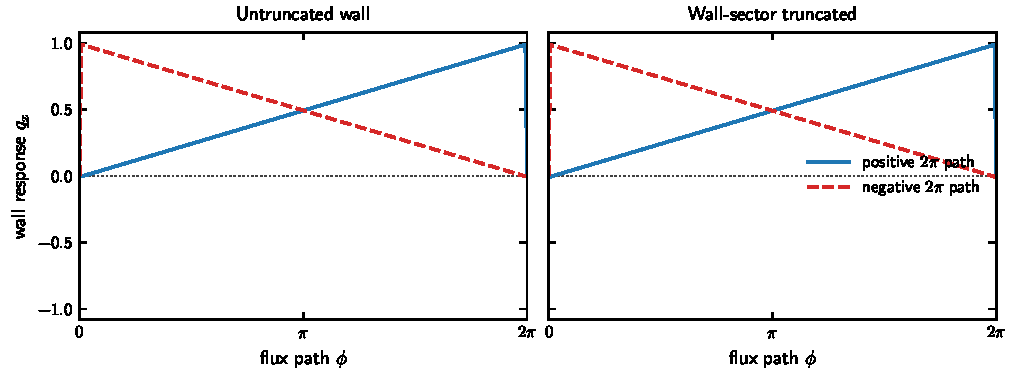
\includegraphics[width=\textwidth]{bare_equilibrium_instantaneous_wall_response_phi.pdf}
  \caption{Bare instantaneous equilibrium response at $20\times40$.  Each
  flux point is filled independently at fixed particle number.  The response
  can be order one near the wall crossing, but the endpoint closes after a
  full flux quantum.}
  \label{fig:eq-instant}
\end{figure*}

The continued family instead leaves one particle--hole rearrangement at the
endpoint.  For the soft wall, increasing flux gives
$(\Delta Q_L,\Delta Q_R,q_x)=(-0.98397186,0.98397186,0.98397186)$, while
decreasing flux gives approximately $(1,-1,-1)$.  The hard-wall values are
$(-0.98080970,0.98080970,0.98080970)$ and $(1,-1,-1)$.  The transferred
density is localized at the two physical interfaces, and reversing the flux
reverses the transfer.  The residual
$|\Delta Q_L+\Delta Q_R|$ is at most $1.14\times10^{-13}$.

\begin{figure*}[t]
  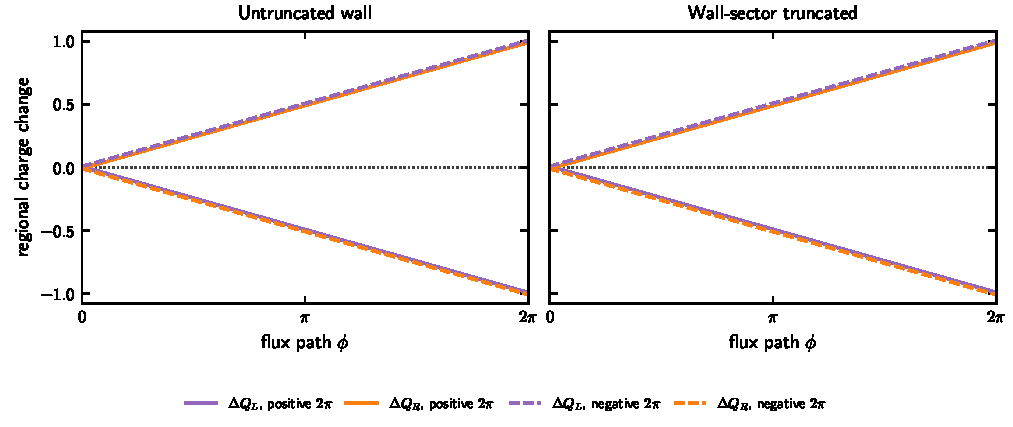
\includegraphics[width=\textwidth]{bare_equilibrium_continued_regional_charge_phi.pdf}
  \caption{Bare continued equilibrium regional charges.  Overlap continuation
  carries the occupied wall branch through the crossing, leaving nearly one
  particle transferred between the two interfaces after one flux quantum.
  Left and right changes are equal and opposite.}
  \label{fig:eq-continued}
\end{figure*}

The finite-size and regulator checks use $N_y=16,24,40$, 65 flux points,
$\phi_0=\pm10^{-7}$, and both soft and hard wall constructions.  With the
quantization-favoring signed origin, the forward magnitudes differ from unity
by at most $2.4\times10^{-9}$ over this size set.  Starting from the opposite
side gives finite-size deficits ranging from $0.00262$ to $0.01919$; the
deficit grows with $N_y$ because the chosen initial branch has a small
opposite-wall component.  A true reverse traversal initialized from the
continued endpoint returns exactly to the initial transported frame within a
projector Frobenius error per dimension below $4.2\times10^{-18}$.  The
flattened Hamiltonian is Hermitian to stored precision, its off-block residual
is below $1.3\times10^{-15}$, and its large-gauge closure error is below
$7.3\times10^{-15}$.

\section{Completed static monitored-circuit response}

\subsection{Protocol}

The monitored calculation uses a $16\times20$ cylinder with topological slab
$x\in[4,12]$.  One soft-wall and one hard-wall trajectory were sampled for 40
cycles from a pure half-filled random state, with random-serial ordering,
perfect correction, no postselection, and complex128 arithmetic.  Each
trajectory's complete zero-twist Born record was then imposed in 68
independent static reruns: 17 twists in each direction for each wall.  The OW
functions and initial state were rebuilt in a common uniform twist gauge for
each rerun.  Neighboring flux points were not dynamically connected.

The signed origin followed Eq.~\eqref{eq:regulated-grid}.  Because each static
rerun imposed the same full record, the total feedback charge was fixed within
an arm: $-2$ for the soft record and $-4$ for the hard record.  The plotted
$\Delta N_L$, $\Delta N_R$, and $q_x$ are direct differences from the
direction-specific origin.  No source-subtracted curve is used in this note.

\subsection{Static-response results}

The two records show substantial wall redistribution.  The maximum response
is
\begin{equation}
  \max_\phi|q_x|=
  \begin{cases}
    0.62806884,&\text{soft wall},\\
    0.43334984,&\text{hard wall}.
  \end{cases}
\end{equation}
The left and right curves are equal and opposite to numerical precision, with
maximum regional-balance residual $8.53\times10^{-14}$.  Global charge
continuity holds to $1.14\times10^{-13}$.  After a full flux quantum, all four
wall/direction paths close: the large-gauge covariance mismatch per dimension
lies between $1.54\times10^{-16}$ and $2.65\times10^{-16}$.

\begin{figure*}[t]
  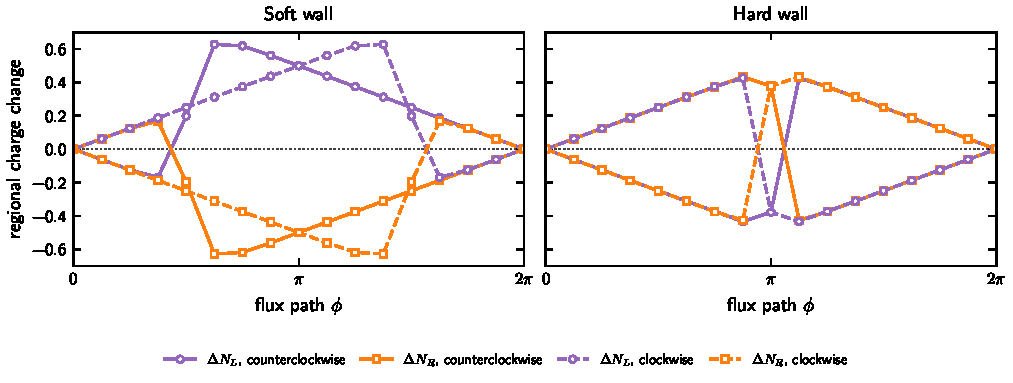
\includegraphics[width=\textwidth]{bare_physical_regional_charge_phi.pdf}
  \caption{Direct regional response of the two completed frozen-record circuit
  trajectories.  Solid/circular and dashed/square curves denote increasing
  and decreasing flux.  Charge moves oppositely between the two half-system
  regions and returns at $2\pi$.}
  \label{fig:static-regional}
\end{figure*}

\begin{figure*}[t]
  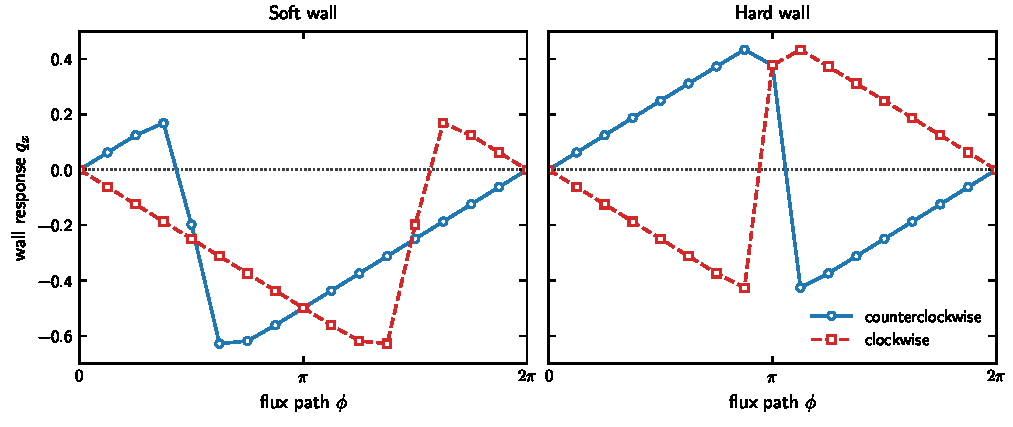
\includegraphics[width=\textwidth]{bare_physical_wall_response_phi.pdf}
  \caption{Bare frozen-record wall response $q_x$ for the soft and hard
  monitored circuits.  Both individual records display an order-one,
  direction-sensitive response, but the closed endpoint distinguishes this
  conditional static family from the continued equilibrium pump.}
  \label{fig:static-qx}
\end{figure*}

The correct present conclusion is consequently narrow but positive: the
conditioned monitored circuit has an order-one, handed wall response in both
wall implementations.  The experiment does not demonstrate transported
charge over a dynamical cycle, because every $\phi$ is a separate static
replay and the state closes at $2\pi$.  The use of only one record per wall is
an additional reason not to infer an ensemble-level pump coefficient.

\section{Preregistered online-ramp pilot}

\subsection{Scientific contract}

The online pilot retains $N_x\times N_y=16\times20$,
$n_{\mathrm{shell}}=1$, $(\alpha_1,\alpha_2)=(1,30)$, pure half filling,
perfect correction, no postselection, and complex128.  It changes the site
order to raster-$y$ and samples ten independent parent trajectories for each
of the soft and hard walls.  Each parent evolves for
$T_{\mathrm{burn}}=2N_y=40$ cycles at exactly zero flux.  Its exact occupied
frame after cycle 40 is then copied into two branches.  The branches share
that physical state but use independently derived random streams for their
subsequent Born outcomes.

For direction $\sigma=+1$ (counterclockwise) or $-1$ (clockwise), the online
schedule is
\begin{equation}
  \phi_0=0,
  \qquad
  \phi_j^{(\sigma)}=\sigma\frac{2\pi j}{16},
  \qquad j=1,\ldots,16.
  \label{eq:online-schedule}
\end{equation}
The OW projectors are rebuilt in the uniform gauge immediately before the
first site update of each ramp cycle.  There is no $10^{-7}$ offset: the online
trajectory starts from the actual zero-flux burn-in state, rather than
selecting a spectral branch at an equilibrium crossing.  The hard-wall branch
is declared already prepared, so its exterior product-state projection is not
applied a second time.

The task table contains 20 burn-ins and 40 ramps.  The two directions for a
given $(\text{wall},\text{sample ID})$ bind to the same burn-in file checksum,
while their continuation seeds are distinct.  Every physical evolution calls
the canonical \code{classA\_U1FGTN.run\_markov\_circuit} entry point; the
campaign runner does not reproduce the Markov loop.

\subsection{Raw and source-corrected observables}

Online perfect correction can change particle number.  For event $e$, let
$m_e\in\{0,1\}$ be the measured OW occupation, $s_e\in\{0,1\}$ its correction
target, and
\begin{equation}
  \delta n_e=s_e-m_e.
\end{equation}
For the normalized OW mode $\lvert\chi_e\rangle$, the cumulative regional
feedback source through ramp cycle $j$ is
\begin{equation}
  A_a(j)=\sum_{e\le j}\delta n_e
  \langle\chi_e|R_a|\chi_e\rangle,
  \qquad a=L,R.
  \label{eq:source}
\end{equation}
The raw changes are referenced to the common branch origin,
$\Delta N_a(j)=N_a(j)-N_a(0)$.  We retain both the requested raw response and
the redistribution after removing the directly assigned feedback source,
\begin{align}
  q_a(j)&=\Delta N_a(j)-A_a(j),\\
  q_x^{\mathrm{corr}}(j)&=\frac{q_R(j)-q_L(j)}{2}.
  \label{eq:corrected}
\end{align}
The event weights must partition unity.  At every cycle boundary the runner
checks
\begin{align}
  \Delta N_{\mathrm{tot}}(j)&=\sum_{e\le j}\delta n_e,\\
  q_L(j)+q_R(j)&=0
\end{align}
to absolute tolerance $10^{-9}$.  Compact products include all 17 values of
$\phi$, raw and corrected regional charges, raw and corrected $q_x$, total
charge, occupied-frame rank, net injection, feedback-event count, continuity
residuals, and the $x$-resolved density and source profile.  No covariance
history is stored.

\subsection{Ensemble analysis and claim boundary}

The independent resampling unit is the wall-specific burn-in sample ID.  The
clockwise and counterclockwise descendants of an ID remain paired in every
bootstrap draw.  The preregistered analysis reports trajectory means and 95\%
trajectory-bootstrap intervals for $\Delta N_{L,R}$, $q_x$, their corrected
counterparts, the direction-odd and direction-even combinations, endpoint
distributions, and wall-resolved density changes.  Direction parity is formed
at common ramp coordinate $|\phi|$:
\begin{equation}
  q_x^{\mathrm{odd/even}}(|\phi|)=
  \frac{q_x^{(+)}(|\phi|)\mp q_x^{(-)}(|\phi|)}{2},
\end{equation}
with the upper sign giving the odd component.

Quantization is not an acceptance criterion.  This is a short, rapidly driven
monitored trajectory with stochastic feedback, not quasistatic continuation
of an equilibrium occupied projector.  The primary questions are whether the
ensemble-averaged response is direction odd, wall localized, reproducible in
both wall constructions, and distinct from its direct feedback source.

\section{Completed continuous frozen-record ramp}

The next calculation isolates flux response from Born sampling noise.  It
reuses, without modification, the twenty verified cycle-40 occupied frames of
the online campaign.  For each wall-specific sample, one further 64-cycle
zero-flux trajectory is generated from that frame and its complete raster-$y$
measurement record $\boldsymbol m$ is frozen.  The same starting frame and the
same prefix of $\boldsymbol m$ are then used for the two directional ramps.
Consequently, the clockwise and counterclockwise descendants have identical
measurement outcomes, correction targets, rank histories, and total injected
charge.  Only their OW functions differ.

For $M\in\{16,32,64\}$ and $\sigma=\pm1$, the ramp is one continuous
conditioned trajectory with
\begin{equation}
  \phi_j^{(\sigma)}=\sigma\frac{2\pi j}{M},
  \qquad j=0,\ldots,M.
  \label{eq:frozen-continuous-schedule}
\end{equation}
The frame at step $j$ is the input to step $j+1$; the calculation never
restarts from the burn-in frame at an intermediate flux.  The first $M$
cycles of the common 64-cycle record are used at ramp length $M$.  There is no
spectral offset because Eq.~\eqref{eq:frozen-continuous-schedule} describes
physical state propagation rather than static eigenstate branch selection.

At all $M+1$ boundaries we save $\Delta N_L$, $\Delta N_R$,
$\Delta N_{\rm tot}$, $q_x$, occupied-frame rank, injection count,
$x$-resolved density, selected-record probability, and numerical continuity
residuals.  No source-subtracted response and no tangent spectrum enter this
experiment.  The primary endpoint test is whether
\begin{equation}
  q_x^{(+)}(2\pi)\simeq-q_x^{(-)}(-2\pi)
\end{equation}
and whether that result stabilizes as $M$ increases.  Integer transfer is not
an acceptance gate.  The independent sampling unit is the frozen record
associated with one burn-in parent; uncertainty bands are one sample standard
deviation across the ten parents.

The campaign contains 20 reference-record tasks and 120 replay tasks.  Each
task writes one atomic NPZ and then a checksum-binding completion JSON.
Restarting verifies those pairs and repeats only missing or invalid tasks.  A
sample-0 pass over both walls and all three ramp lengths precedes the remaining
ensemble, but contributes directly to the same production output rather than
forming a separate scientific sample.
The versioned output root is
\code{results/N16x20\_frozen\_record\_continuous\_ramp\_s10\_v1}, with root
seed \code{2026090302}.  The launch uses 28 one-thread workers on physical
cores 28--55, leaving the modular-handedness campaign on cores 0--27
untouched.

\subsection{Continuous-ramp results}

All 20 reference records and all 120 ramp products passed checksum and pairing
verification.  The largest charge-continuity residual was
$1.08\times10^{-11}$.  Define the paired direction-odd endpoint by
\begin{equation}
 q_{x,\mathrm{odd}}(M)=
 \frac{q_x^{(+)}(2\pi)-q_x^{(-)}(-2\pi)}{2}.
\end{equation}
For the soft wall its mean and sample standard deviation at
$M=(16,32,64)$ are $(0.7122\pm0.2234,0.4959\pm0.1513,
0.1475\pm0.1655)$.  The hard-wall values are
$(0.9139\pm0.0932,0.7415\pm0.1930,0.3199\pm0.1927)$.
The signal is handed and reproducible at the faster ramps, but decreases as
the ramp is slowed.  In this accessible range it therefore does not approach
a nonzero quantized adiabatic pump.

\begin{figure*}[t]
  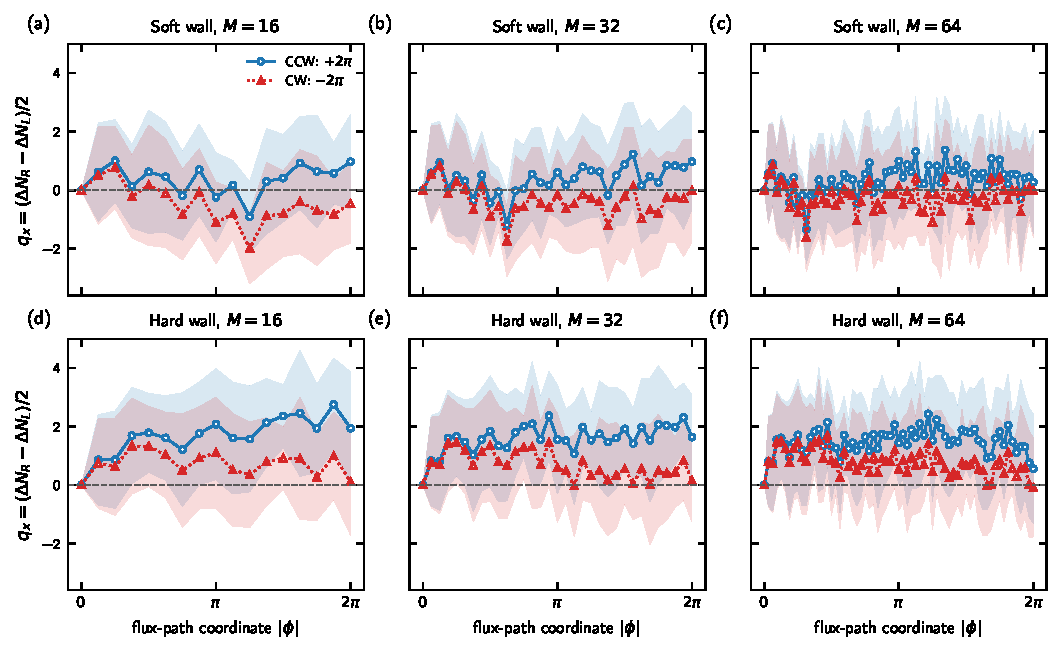
\includegraphics[width=\textwidth]{frozen_continuous_ramp_qx.pdf}
  \caption{Direct continuously replayed frozen-record response for ten paired
  records per wall.  Curves show trajectory means and shading denotes one
  sample standard deviation.  The same ordered outcomes are imposed in the
  two directions at each $M$.}
  \label{fig:continuous-frozen-qx}
\end{figure*}

\section{Preregistered fixed-flux quench}

The next calculation asks a distinct nonadiabatic question.  For each of the
same 20 burn-in frames and 64-cycle records, the frame is reset and every OW
projector in the replay is held at
\begin{equation}
 \phi=\sigma\varphi,\qquad
 \varphi\in\left\{\frac{\pi}{2},\pi,\frac{3\pi}{2},
 2\pi-10^{-7}\right\},\qquad \sigma=\pm1.
 \label{eq:fixed-flux-grid}
\end{equation}
The constant schedule is installed before the cycle-zero observation and
remains unchanged for all 64 cycles.  This is a sudden change of the
measurement channel, not a ramp.

Let $N_a^{\phi}(t)$ be the half-system charge obtained from the fixed-twist
replay and $N_a^0(t)$ the charge in the zero-flux generation of the same
record.  The direct paired response is
\begin{align}
 \delta_\phi N_a(t)&=N_a^{\phi}(t)-N_a^0(t),\\
 q_x^{\phi}(t)&=\frac{\delta_\phi N_R(t)-\delta_\phi N_L(t)}{2}.
 \label{eq:fixed-flux-response}
\end{align}
Equation~\eqref{eq:fixed-flux-response} is a same-record state difference; it
is not a subtraction of an analytically assigned feedback source.  Clockwise
and counterclockwise partners have identical records, rank histories, and
feedback-injection histories.  The paired odd response
$[q_x^{+\varphi}(t)-q_x^{-\varphi}(t)]/2$ is primary, while the even component
diagnoses record-specific redistribution.

The near-$2\pi$ point tests large-gauge closure after a sudden projector
quench.  A small response would establish that the fixed channel remains
periodic; a transient response would quantify the failure of the untwisted
burn-in state to be stationary under the gauge-shifted conditioned channel.
Neither outcome is interpreted as an adiabatic or quantized pump.  The
campaign contains 160 atomic replay tasks, uses root seed
\code{2026090303}, and writes to
\code{results/N16x20\_frozen\_record\_fixed\_flux\_quench\_s10\_v1}.

\section{Completed finite-difference parent-Hamiltonian ramp}

\subsection{State-derived Hamiltonian and physical evolution}

The static projector continuation above answers which occupied subspace is
obtained by following eigenmodes through a flux crossing; it does not solve a
time-dependent Schr\"odinger equation.  To make that distinction operational,
we reuse 50 verified endpoints from the completed
$N_x\times N_y=20\times24$ monitored ensemble: sample IDs
$0,4,\ldots,96$ for each of the soft and hard walls.  This every-fourth-ID
selection was fixed independently of the earlier zero/unit pump outcome.

For each endpoint occupied frame $F_0$, define
\begin{equation}
 P_0=F_0F_0^\dagger,
 \qquad h_0=\mathbf{1}-2P_0.
 \label{eq:rk-parent}
\end{equation}
The entire Hamiltonian path is constructed from this fixed $h_0$; it is not
rebuilt from the evolved state.  With minimum-image periodic displacement
$d_y(r,s)$, the threaded parent is
\begin{equation}
 h_{rs}(\phi)=
 (h_0)_{rs}\exp\!\left[\ii\phi\frac{d_y(r,s)}{N_y}\right],
 \label{eq:rk-twist}
\end{equation}
followed by explicit Hermitian symmetrization at roundoff level.  The flux is
ramped in both orientations,
\begin{equation}
 \phi_\sigma(t)=\sigma\frac{2\pi t}{T},
 \qquad \sigma=\pm1,\qquad T=10^4,
 \label{eq:rk-schedule}
\end{equation}
and the occupied frame obeys
\begin{equation}
 \ii\frac{dF}{dt}=h[\phi_\sigma(t)]F.
 \label{eq:rk-schrodinger}
\end{equation}
This is deterministic unitary evolution under a constructed one-particle
parent Hamiltonian.  It is neither a rerun of the monitored circuit nor an
instantaneous spectral reprojection.

\subsection{Finite-difference scheme and observables}

Equation~\eqref{eq:rk-schrodinger} is integrated in complex128 using classical
explicit fourth-order Runge--Kutta with the Hamiltonian evaluated at the
beginning, midpoint, and end of every step.  The loop contains 128 equal-flux
observation intervals and 320 RK4 steps per interval, hence 40960 steps and
\begin{equation}
 \Delta t=\frac{10^4}{40960}=0.244140625.
\end{equation}
At observation boundaries a thin QR factorization removes accumulated
occupied-frame gauge and norm error.  Right-unitary changes of $F$ leave
$FF^\dagger$ invariant, so this stabilization is not an energetic
reprojection.  Maximum Gram residuals are retained before and after every QR.

At all 129 observation points we save $\phi$, $t$, $\Delta N_L$,
$\Delta N_R$, $q_x$, total-charge residual, $x$-resolved density, instantaneous
left current, and parent-Hamiltonian expectation value.  Endpoint diagnostics
include overlap with the large-gauge-transformed source frame, overlap with
the independently filled instantaneous occupied subspace, its excitation
number, and the instantaneous occupied--empty gap.  Each of the 100
wall/direction paths writes one compact result/completion pair.  Because a
single path is long, one rolling occupied-frame checkpoint is updated every
four flux intervals; a restart repeats at most that interval block.

The production discretization is checked by an independent four-path
step-halving calculation using sample 0 for both wall constructions and both
orientations.  That calculation uses 640 RK4 steps per observation interval,
$\Delta t=0.1220703125$, and a separate configuration and output root.  We
compare both the endpoint and the maximum pointwise difference in $q_x$; the
four paths are a numerical convergence test and are not included as additional
statistical samples.

\subsection{Finite-size crossing prediction and observed response}

At finite circumference the wall crossing is generally avoided.  The
strictly slow limit can therefore follow the instantaneous occupied subspace
through the avoided crossing and return to the original charge distribution,
whereas diabatic passage can remain on the spectral-flow branch and leave an
order-one $q_x$.  In a local two-level approximation with minimum gap $g$ and
crossing slope $s$, the diabatic probability is
\begin{equation}
 P_{\rm D}\simeq
 \exp\!\left(-\frac{Tg^2}{4s}\right).
 \label{eq:lz-prereg}
\end{equation}
This formula was preregistered as a descriptive comparison, not an acceptance
gate.  Five-point fits to the already saved gap curves give median
$s=0.74282$ for the selected soft states and $0.74296$ for the hard states,
with interquartile widths below $0.002$.  Before any RK4 path completed,
Eq.~\eqref{eq:lz-prereg} predicted $P_{\rm D}>1/2$ for 16 of 25 soft states
and 13 of 25 hard states.  The primary analysis tests the endpoint
direction-odd $q_x$ against this gap prediction and against each state's prior
static continued-projector classification.  Neither integer transfer nor
adiabatic closure was imposed as an acceptance criterion.  All 100 paths are
now checksum verified.  The raw soft-wall endpoint means are $q_x=+0.71569$
for CCW and $-0.71422$ for CW; 18 of 25 paths in each direction have
$|q_x|>0.5$.  For the hard wall the corresponding means are $+0.53622$ and
$-0.53624$, with 13 of 25 paths above $0.5$ in each direction.  Charge
conservation is better than $2.6\times10^{-13}$ and the maximum post-QR Gram
residual is $2.7\times10^{-14}$.  The endpoint response is strongly sample
dependent and nearly antisymmetric under direction reversal.

To distinguish transport from final finite-size closure, the preregistered
summary reports three quantities for each saved endpoint: the direction-odd
$q_x$ at $|\phi|=\pi$, the largest $|q_x|$ attained anywhere along the loop
and its flux location, and the residual direction-odd $q_x$ at $|\phi|=2\pi$.
Endpoint paths are described as closed when $|q_x|<0.25$, order-one when
$|q_x|>0.75$, and intermediate otherwise; these labels summarize the
distribution and are not pass/fail thresholds.

\subsection{Canceled physical-time width repeat}

The sample-dependent avoided-crossing interpretation was to be tested by
increasing only the separation between the two walls.  A second calculation
reused 25
soft-wall and 25 hard-wall endpoints from the completed
$N_x\times N_y=24\times24$ monitored ensemble, again selecting IDs
$0,4,\ldots,96$ without reference to their static pump outcomes.  Its walls
are at $x=6,18$, so both separations equal 12 sites, compared with 10 sites in
the $20\times24$ calculation.  The circumference, flux grid, ramp time,
Runge--Kutta step, wall definitions, subsystem partition at $N_x/2$, and all
analysis thresholds remain unchanged.  Because the two geometries were
generated with independent monitored-trajectory seeds, directions are paired
within each endpoint but statistical comparisons between $N_x=20$ and 24 are
unpaired.

Before any $24\times24$ RK4 path was evaluated, its saved static continuation
data gave 23 of 25 soft-wall events and 11 of 25 hard-wall events under
$|q_x^{\rm odd}(2\pi)|>0.5$.  The corresponding mean static responses are
$0.91588$ and $0.43988$, while the median minimum occupied--empty gaps are
$0.00898$ and $0.01738$.  These values and the complete endpoint selection are
stored in a checksum-bound preregistration record.  The test asks whether the
larger wall separation shifts the gap distribution, the direction-odd charge
distribution, or the fractions above $0.5$ and $0.75$.  None is an acceptance
gate.

The physical-time $24\times24$ run was stopped on September 6, 2026, because
the scientific question was replaced by geometric Kato continuation.  At the
stop, no path had completed, 28 rolling NPZ/JSON checkpoint pairs were
verified, every checkpoint was at observation interval 104 of 128, and 72
paths had not started.  The configuration, log, and all checkpoints remain in
the original versioned output directory.  The exact inventory is recorded in
\code{cancellation\_inventory.json}; the stopped artifacts are not interpreted
as results and are not overwritten.

\section{Preregistered adaptive Kato continuation}

The replacement width experiment transports the overlap-selected spectral
projector geometrically rather than evolving a state in physical time.  It
uses the same endpoint IDs at $20\times24$ and $24\times24$, both walls, and
both flux orientations.  At every RK4 stage, eigenvectors of the twisted
state-derived parent are ranked by their previous-projector weights; the
fixed-rank selected projector supplies the analytic Kato generator
$[\partial_\phi P_{\rm spec},P_{\rm spec}]$.  One full step is compared with
two half steps and accepted only when their normalized projector discrepancy
is at most $10^{-8}$.  The selected--excluded gap is saved, but does not alone
choose the step.

The complete theory, derivation from $P^2=P$, analytic projector derivative,
adaptive controller, regulator convention, diagnostics, and resume protocol
are fixed in the companion two-column methods note
\code{kato\_overlap\_continuation\_methods.tex}.  The campaign contains 200
paths and reports raw CW and CCW $q_x$ separately.  Quantization, agreement
with the 64- and 128-grid static classifications, and width dependence are
pending measured outcomes, not acceptance gates.


\section{Completed wall-diabatized spectral flow of monitored endpoints}

The final spectral calculation uses the same direct regional charge as
Eq.~\eqref{eq:qx}, but changes how the occupied subspace is continued at the
rank crossing.  The input matrix contains $N_y=24$ and
$N_x=20,24,28,32$, soft and hard walls, and both $n_{\rm shell}=1$ and the
dense OW construction.  Each of the 16 $(n_{\rm shell},N_x,{\rm wall})$
cells contains $S=100$ independent pure, half-filled monitored endpoint
states prepared for 48 raster-$y$ cycles with perfect correction and no
postselection.  No monitored dynamics is rerun during flux threading.

For every endpoint projector, the single-particle parent is threaded through
256 intervals in each direction.  Ordinary occupied spectator states are
continued by previous-projector overlap.  The two modes at the occupied--empty
boundary are removed from that global assignment, their isolated cluster is
aligned between neighboring flux points, and
$E^\dagger(R_R-R_L)E$ defines left- and right-localized wall modes.  The wall
label occupied on entering the crossing is retained through it and then
recombined with the spectator subspace.  A path is marked unresolved when the
pair is not isolated or oppositely wall localized, but unresolved paths remain
in every raw distribution and mean below.

Figures~\ref{fig:working-mean-nsh1} and~\ref{fig:working-mean-dense} show the
complete flux-resolved response.  CCW and CW are plotted separately; no
$q_x^{\rm odd}$ combination is used.  The curves expose an almost linear
spectral transfer from zero to the orientation-expected unit response.  The
standard-deviation bands are controlled mainly by a small zero-transfer
subpopulation rather than by broadly fractional sample-wise responses.

Figure~\ref{fig:working-chirality-nx32-hard-nsh1} isolates the requested
chirality diagnostic: the raw right-subsystem charge at $N_x\times N_y=
32\times24$ for the hard wall and $n_{\rm shell}=1$ only.  CW is placed on the
negative signed-flux axis and CCW on the positive signed-flux axis.  The
vertical error bars are the standard error of the mean, $s/\sqrt{100}$,
rather than a confidence interval.  Separate zero-intercept least-squares
fits use $\langle\Delta N_R\rangle=m\phi/(2\pi)$ and give
$m=0.9647$, $R_0^2=0.999988$ for CCW and
$m=0.9659$, $R_0^2=0.999987$ for CW.

\begin{figure}[t]
 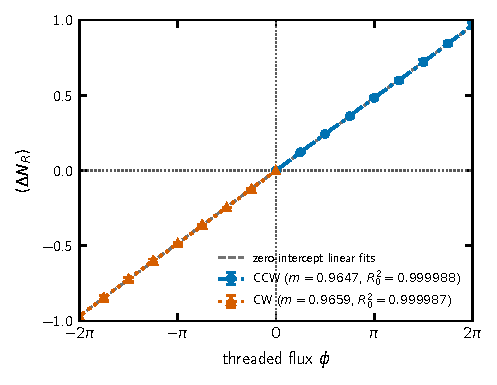
\includegraphics[width=\columnwidth]{../results/N20_24_28_32x24_wall_diabatic_spectral_pump_reconciled_v1_v2/analysis/figures/reconciled_Nx32_hard_nsh1_mean_delta_N_right_vs_signed_flux_sem.pdf}
 \caption{Chiral right-subsystem charge response for the $32\times24$ hard
 wall with $n_{\rm shell}=1$.  The curves show the raw trajectory mean
 $\langle\Delta N_R\rangle$ for $S=100$ independent endpoint states per
 direction, and the vertical bars show $\pm$SEM.  The signed axis displays CW
 on $-2\pi\leq\phi\leq0$ and CCW on $0\leq\phi\leq2\pi$.
 Charge conservation gives $\Delta N_L=-\Delta N_R$ to numerical precision,
 so the redundant left-subsystem curve is omitted.  Gray dashed segments are
 separate zero-intercept fits in normalized signed flux; the corresponding
 slopes and through-origin coefficients of determination are reported in the
 legend.}
 \label{fig:working-chirality-nx32-hard-nsh1}
\end{figure}

\begin{figure*}[t]
 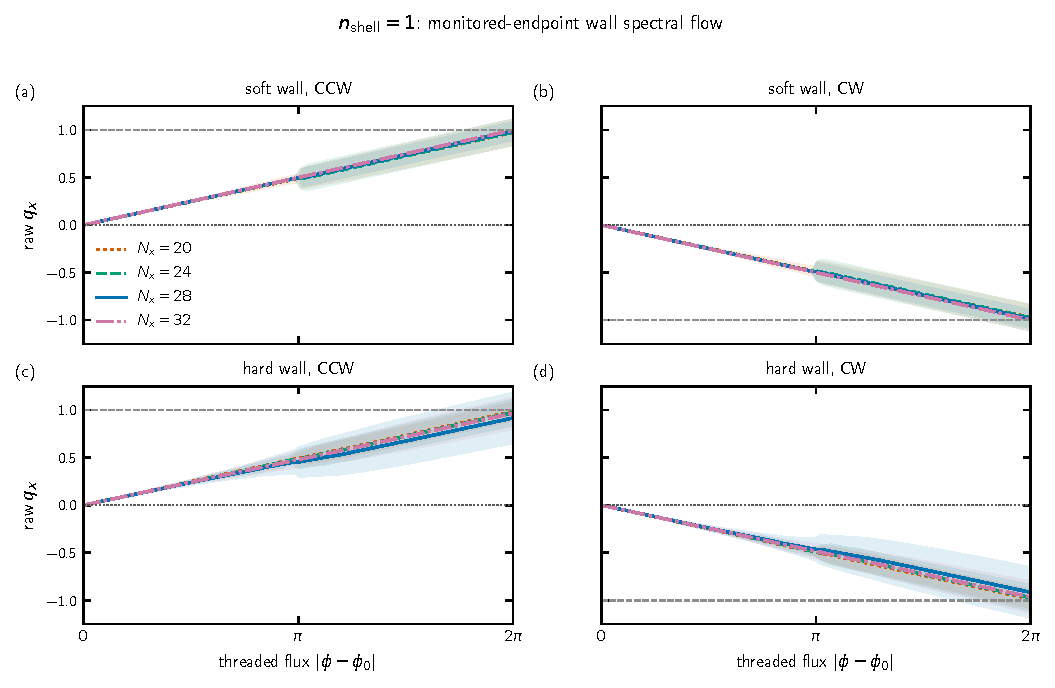
\includegraphics[width=\textwidth]{../results/N20_24_28_32x24_wall_diabatic_spectral_pump_reconciled_v1_v2/analysis/figures/reconciled_mean_qx_vs_flux_nsh1.pdf}
 \caption{Raw flux-resolved wall response for $n_{\rm shell}=1$.  Rows show
 soft and hard walls and columns show CCW and CW paths.  Each curve is the mean
 of $S=100$ independent monitored endpoint states at fixed $N_x$; shaded bands
 are one trajectory standard deviation.  Colors and line styles distinguish
 $N_x=20,24,28,32$ at fixed $N_y=24$.  Every source trajectory starts from a
 pure half-filled state and runs for 48 raster-$y$ cycles.  The estimator is
 the 256-interval wall-diabatized spectral continuation, and unresolved paths
 are retained.}
 \label{fig:working-mean-nsh1}
\end{figure*}

\begin{figure*}[t]
 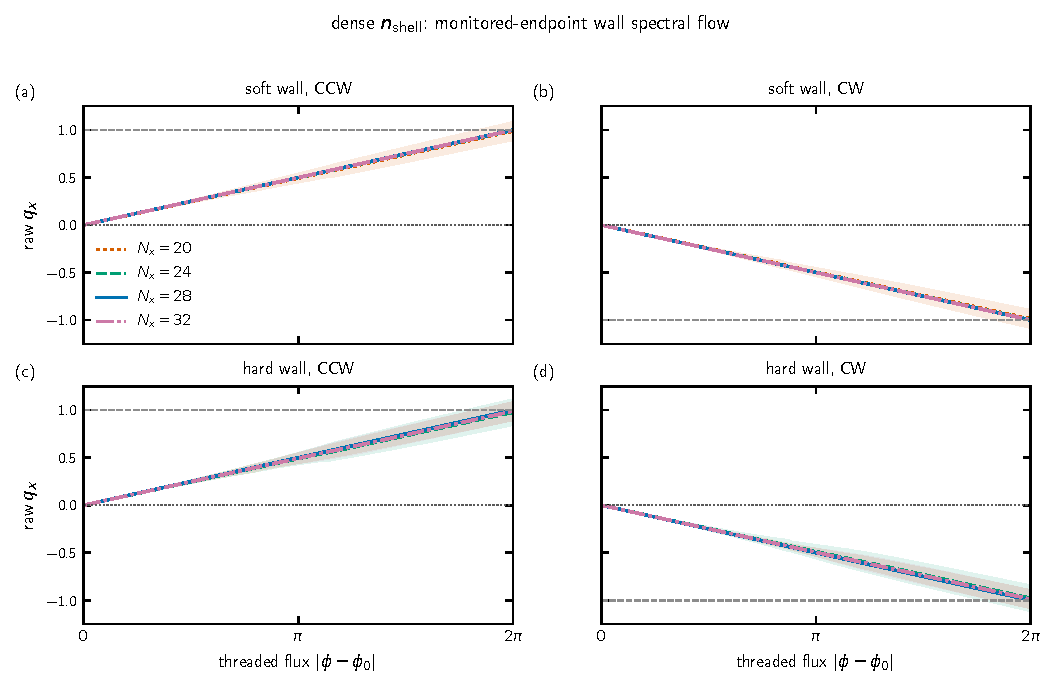
\includegraphics[width=\textwidth]{../results/N20_24_28_32x24_wall_diabatic_spectral_pump_reconciled_v1_v2/analysis/figures/reconciled_mean_qx_vs_flux_dense.pdf}
 \caption{Raw flux-resolved wall response for the dense OW construction, with
 the same geometry, initialization, 48-cycle preparation, 256-interval
 estimator, $S=100$ independent sampling unit, and trajectory-standard-
 deviation uncertainty as Fig.~\ref{fig:working-mean-nsh1}.  Dense soft-wall
 curves at $N_x=28,32$ are nearly coincident and reach unit response with
 negligible inter-trajectory spread.}
 \label{fig:working-mean-dense}
\end{figure*}

Of the 3200 directional paths, 3145 (98.3\%) have the correct orientation and
$|q_x|>0.9$; 3120 (97.5\%) satisfy
$0.95\leq|q_x|\leq1.05$.  Forty-eight paths (1.5\%) lie within $0.1$ of zero,
and only seven lie between the near-zero and near-unit sectors.  The broadest
cell is the $n_{\rm shell}=1$ hard wall at $N_x=28$, with raw endpoint means
$+0.9177$ for CCW and $-0.9174$ for CW.  The dense soft-wall cells at
$N_x=28,32$ give unit response for all 200 directional paths at each width to
the displayed precision.  The wall cluster is qualified for 1569 of 1600
endpoints; the 31 unresolved endpoints are retained in these numbers.

The maximum total-charge residual over the reconciled matrix is
$4.55\times10^{-13}$, the maximum frame/projector residual is
$9.59\times10^{-14}$, and the largest forward--reverse undo error is
$2.33\times10^{-15}$.  Thus the small non-unit population is not numerical
charge leakage.  The improvement over the earlier binary ordinary-overlap
calculation comes from specifying the wall branch inside an independently
qualified edge cluster, rather than allowing the global rank selector to make
a grid-sensitive choice at the finite-size avoided crossing.

The executable companion
\path{notebooks/equilibrium_wall_crossing_explorer/equilibrium_wall_crossing_explorer.ipynb}
uses a deterministic translation-invariant $20\times24$ equilibrium OW slab
to expose this crossing with two flux sliders.  It displays the energy
splitting, exchange of left/right character, wall-localized basis, instantaneous
and continued occupations, and direct $q_x$.  Its saved default run gives
$q_x(2\pi)=0.9999999992$ for overlap continuation while instantaneous refilling
closes within $3.5\times10^{-10}$.

\section{Execution, provenance, and status}

Each fixed-flux replay writes one compressed NPZ followed by one small
completion JSON.  The completion record binds task ID, wall, sample ID, fixed
twist, seed, scientific configuration hash, source hashes, result byte count,
and SHA-256, as well as the exact burn-in and reference-record SHA-256 values.
Restart verifies both members and reruns only a missing or invalid task.  There
is no intra-task checkpoint, server transaction layer, migration ledger, or
background Drive telemetry.

The fixed-flux production root is
\code{results/N16x20\_frozen\_record\_fixed\_flux\_quench\_s10\_v1}.
The root seed is \code{2026090303}.  The host launch uses 28 single-thread workers on physical
cores 28--55 and leaves the modular-handedness calculation on cores 0--27
untouched.  Progress bars report completed replay cycles and tasks.  Analysis
begins only after all 160 replay products verify.

\begin{table}[b]
\caption{Campaign status when the fixed-flux quench was preregistered.
``Pending'' is a statement about saved
products, not a physical result.}
\begin{ruledtabular}
\begin{tabular}{lcc}
calculation & independent samples & status\\
\colrule
exact flattened Hamiltonian & deterministic & complete\\
static frozen record & 1 soft + 1 hard & complete\\
online ramp burn-in & 10 soft + 10 hard & complete\\
online $\pm2\pi$ ramps & 20 per direction & complete\\
continuous frozen records & 10 soft + 10 hard & complete\\
continuous frozen ramps & 60 per direction & complete\\
fixed-flux quenches & 80 per direction & pending\\
$20\times24$ physical-time RK4 & 50 states, 2 directions & complete\\
$24\times24$ physical-time RK4 & 50 states, 2 directions & canceled (28 checkpoints)\\
adaptive Kato width test & 100 states, 2 directions & pending\\
wall-diabatized spectral width sweep & 1600 states, 2 directions & complete\\
\end{tabular}
\end{ruledtabular}
\end{table}

No statement about the sign, magnitude, quantization, or width dependence of
the adaptive Kato result is made before those products exist.  All earlier
results and the canceled physical-time checkpoints are preserved in their
original versioned directories and are not overwritten by this campaign.

\bibliography{references}

\end{document}
